\subsection{KNN Reduction Results}
In this section we will discuss the results obtained when training and testing KNN models on reduced versions of the folds from our 2 original datasets, in order to perform statistical analyses on the reduction methods and extract conclusions about their different impact on classifier performance.

We perform this experiment separately for the Hepatitis and Mushroom datasets, and for each of them we employ the KNN model configuration that we concluded to be the best for that dataset, in Section \ref{sec:res:knn}. We first train and test the corresponding KNN models over the original folds of the datasets, and then we repeat the process over the reduced folds for each of the 3 reduction methods: GCNN, EENTH, and DROP3. We store this evaluation data in a CSV for each of the datasets, for its later evaluation and statistical analysis.

\subsubsection{Hepatitis}
Before starting the statistical analysis, let us first look at the results, summarized in Figure \ref{fig:hep:reduction}, where we can see the accuracy distributions per reduction method (in boxplots) and the storage percentage comparison, against the ``no-reduction method'' (i.e. \texttt{NONE}). The storage percentage refers to the percentage of samples each of the reduction methods keeps from the original folds.
\begin{figure}[H]
    \centering
    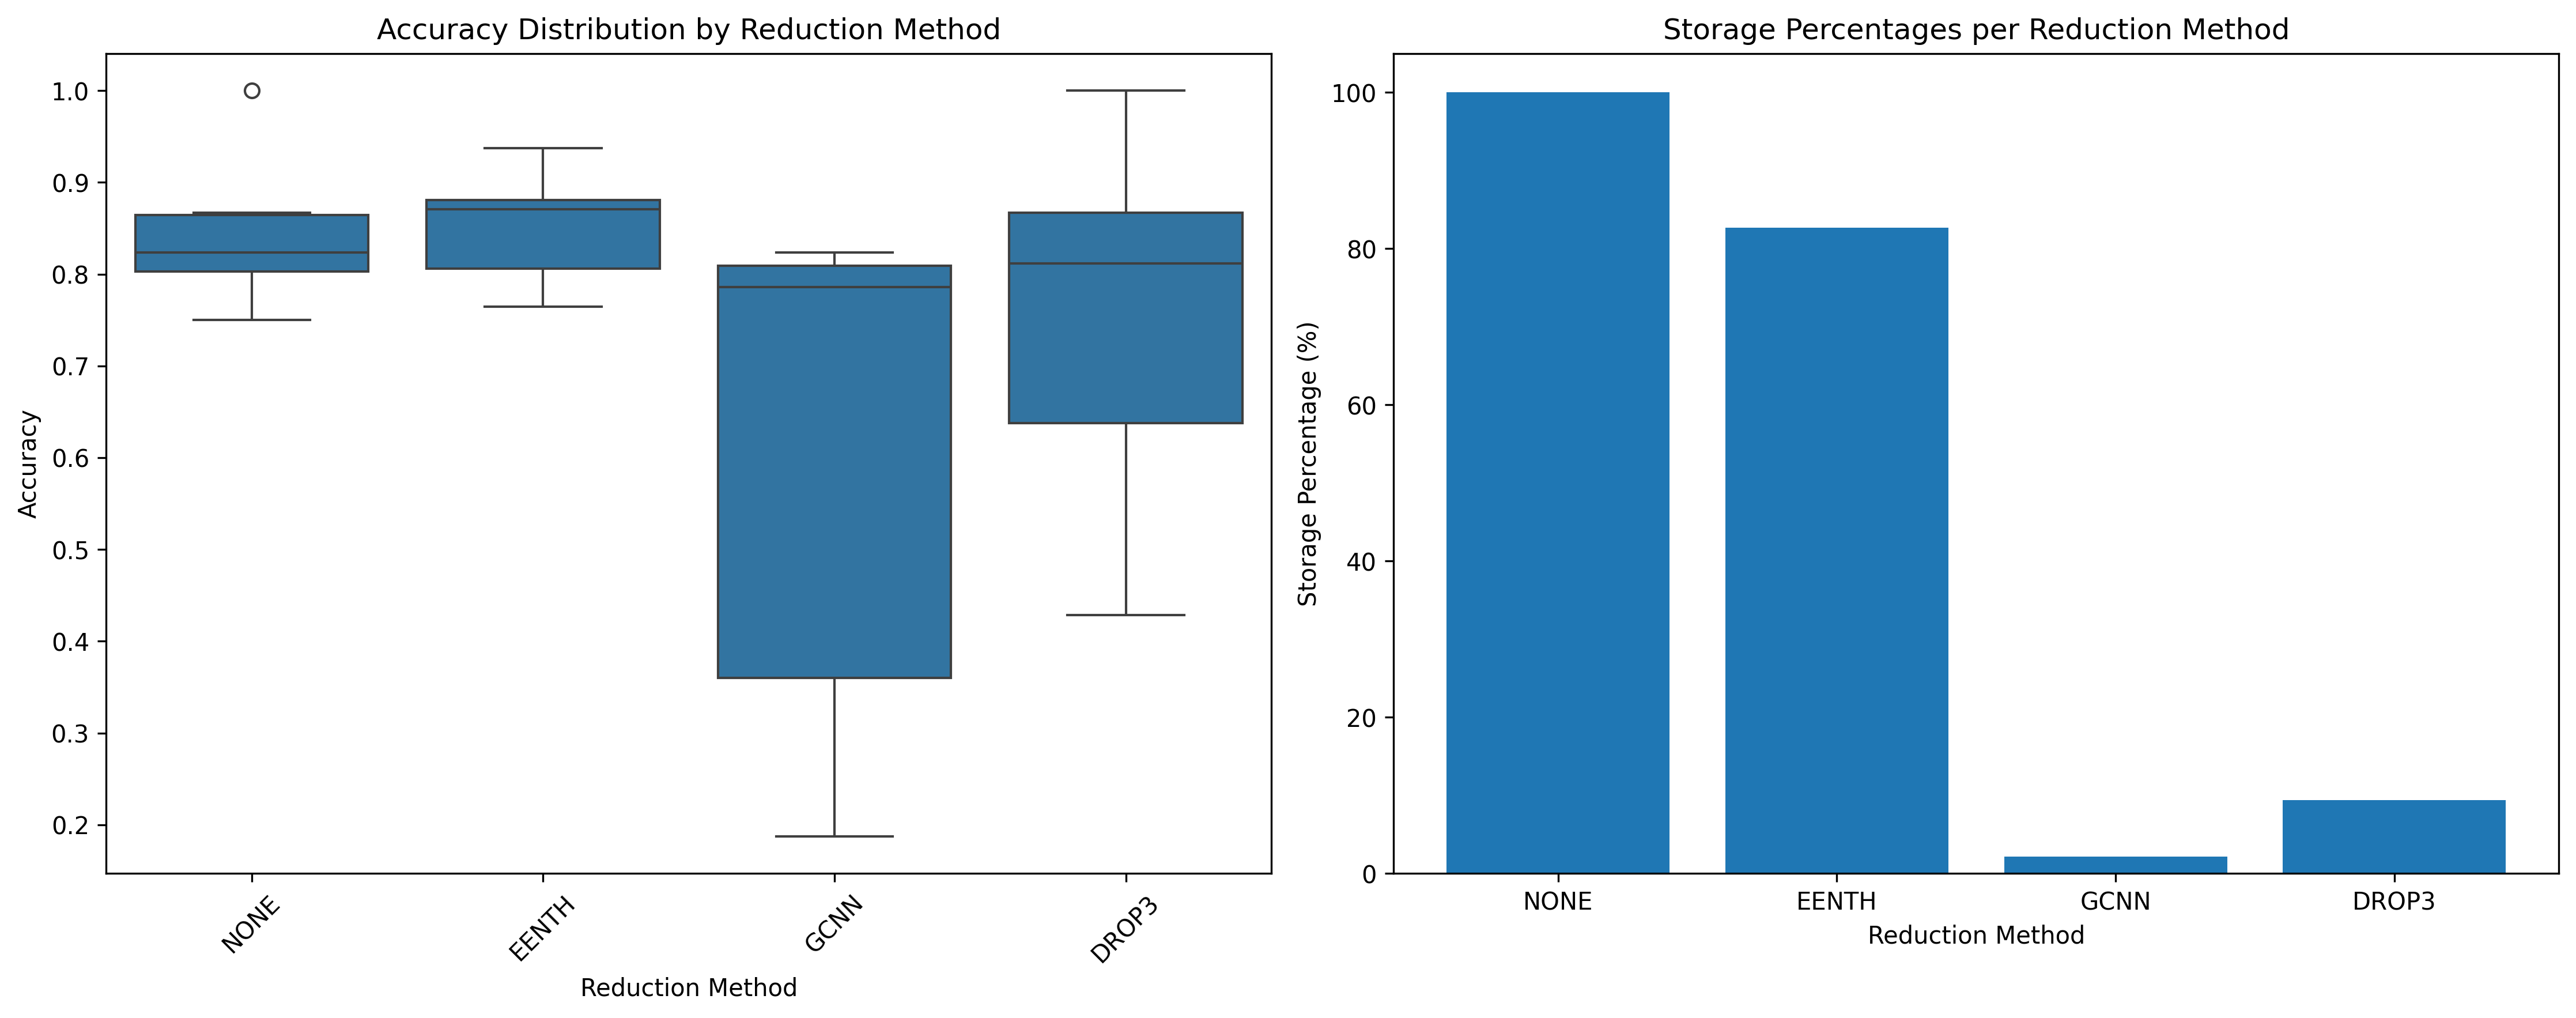
\includegraphics[width=\textwidth]{figures/knn/hepatitis/accuracy_storage_comparison.png}
    \caption{Hepatitis accuracy and storage comparison}
    \label{fig:hep:reduction}
\end{figure}

We observe that the DROP3 reduction method is the most inconsistent of them, with a very wide accuracy distribution, followed by the GCNN method, which is more consistent but not as accurate as NONE and EENTH. Interestingly, these 2 methods (GCNN and DROP3) are also the most radical ones in terms of reduction of samples, which is clearly shown in the Storage Percentage graph. We can start to see a trend where the more extreme the reduction percentage, the more inconsistent the models performance; which is an intuitive deduction, since we lose information when reducing samples.

We now proceed with the statistical analysis to study whether there are significant differences between the impact of each reduction method on the performance of the KNN classifier. For this, we apply a Friedman test on the results, grouping by reduction method. The p-value that we obtain from this test is \textbf{0.0093}; hence, if we establish a level of significance of $ \alpha = 0.15 $, we can reject the null-hypothesis and state that \uline{there are indeed statistically significant differences between the performances of the classifier when applying the different reduction methods}.

The next step is performing a post-hoc test to determine among which of the reduction methods there are significant differences. There is an obvious ``control'' reduction method, which is no-reduction, so we apply a Bonferroni test to study the differences of each of the other reduction methods when compared to the original training sets. The results are displayed on Table \ref{tab:knn:hep:red-posthoc}.

\begin{table}[h!]
    \centering
    \small
    \begin{tabular}{|l|c|c|}
    \hline
                             & \textbf{p-value} & \textbf{Difference in accuracy (\%)} \\ \hline
    \textbf{EENTH} & 1.0000           & 2.2288\%          \\ \hline
    \textbf{GCNN}           & 0.0527           & -9.3174\%          \\ \hline
    \textbf{DROP3}           & 0.4140           & -9.4072\%          \\ \hline
    \end{tabular}
    \caption{Results of the Bonferroni post-hoc test}
    \label{tab:knn:hep:red-posthoc}
\end{table}

From these results we can extract multiple conclusions. For one, we see that on average the EENTH reduction method seems to have slightly better accuracy than the control; however, the p-value of \textbf{1.000} indicates that this difference could be due to pure chance, and it is not meaningful at all. On the other hand, the GCNN obtains a p-value of \textbf{0.0527}, which means that we can state with our level of significance of $ \alpha = 0.15 $ that there are statistically significant differences with the control; and the negative difference in accuracy percentage indicates that these differences are against using GCNN over the control. Lastly, DROP3 shows worse performance than no-reduction, but the p-value of \textbf{0.4140} indicates that this decline in classification performance is not too significant, and could be due to randomness or noise in the data.

The final conclusion of these results is that, for the Hepatitis dataset, \uline{the GCNN reduction method causes significantly worse classification performance than not reducing the data, while the other 2 reduction methods show no meaningful difference}.

\subsubsection{Mushroom}
In this section we will follow for the Mushroom dataset the same procedure as we did in the previous section for the Hepatitis dataset; starting with a plot to summarize the results (Figure \ref{fig:mush:reduction}).
\begin{figure}[H]
    \centering
    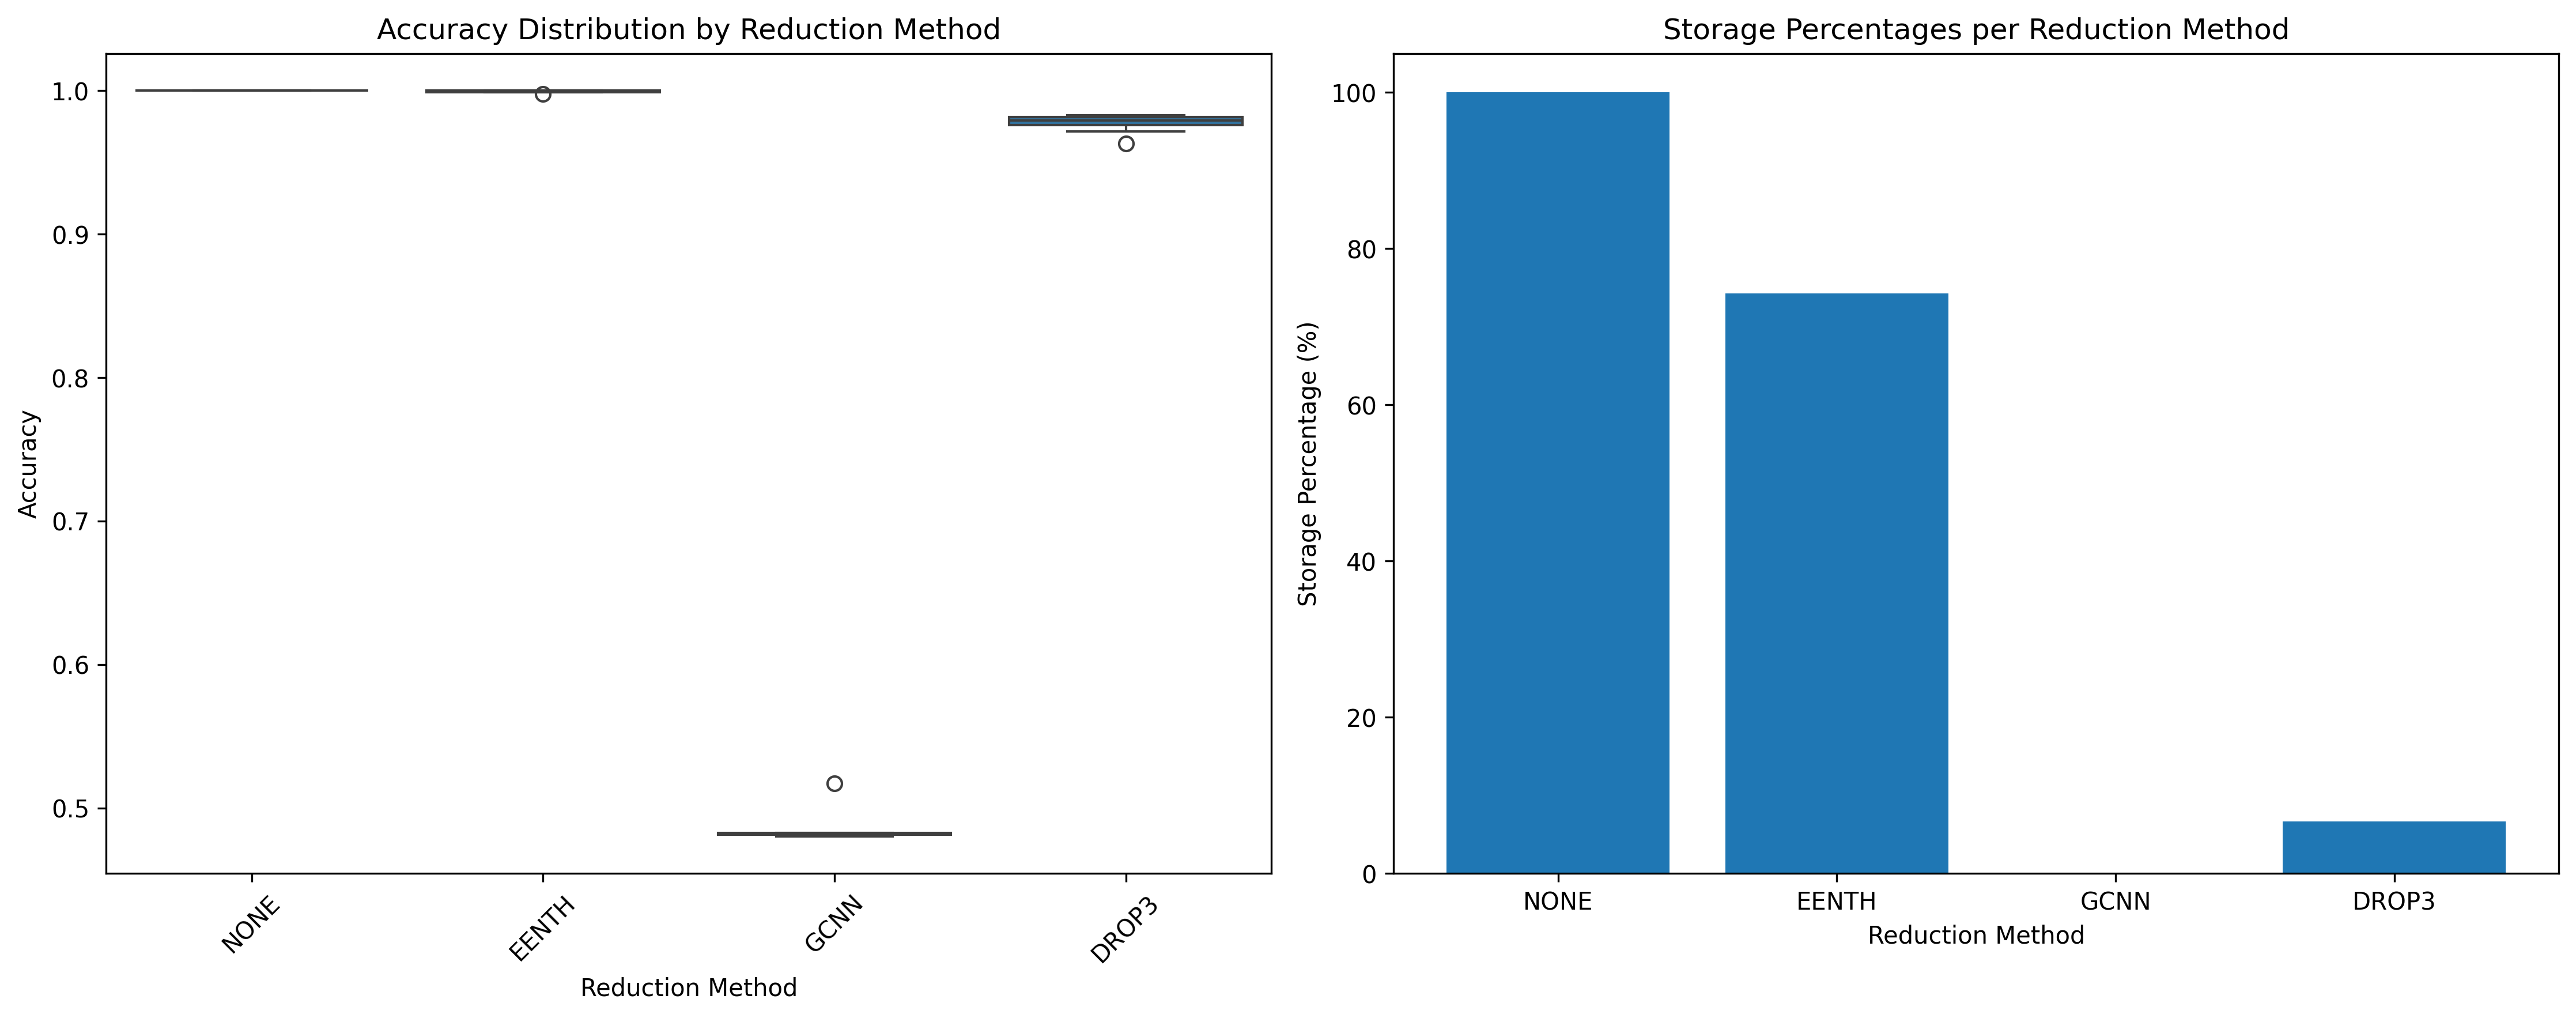
\includegraphics[width=\textwidth]{figures/knn/mushroom/accuracy_storage_comparison.png}
    \caption{Mushroom accuracy and storage comparison}
    \label{fig:mush:reduction}
\end{figure}

Although the plots seem more radicalized than for the Hepatitis dataset (due to extremely high performance of the classifier), they still follow a similar trend as for the Hepatitis dataset, which supports the idea that as the reduction gets more intense, the KNN performance declines. This time, however, we can observe an extreme difference (relatively, since all achieve accuracy over 0.9) between the GCNN and the other 3 methods, which might indicate that it is especially not suitable for this specific dataset. The DROP3 seems to keep a reasonable performance while achieving a high storage reduction percentage.

After applying the Friedman test on the results we obtain a p-value of \textbf{0.000}, which strongly suggests we can reject the null-hypothesis with any level of significance. Therefore, we deduce that \uline{there is indeed significant differences in classification performance on the Mushroom dataset with the different reduction methods}.

Again, we perform a Bonferroni post-hoc test to further study these differences, comparing against the control (no-reduction). The results are shown in Table \ref{tab:knn:mush:red-posthoc}.
\begin{table}[h!]
    \centering
    \small
    \begin{tabular}{|l|c|c|}
    \hline
                             & \textbf{p-value} & \textbf{Difference in accuracy (\%)} \\ \hline
    \textbf{EENTH} & 0.3264           & -0.0493\%          \\ \hline
    \textbf{GCNN}           & 0.0059           & -8.2349\%          \\ \hline
    \textbf{DROP3}           & 0.0059           & -2.2644\%          \\ \hline
    \end{tabular}
    \caption{Results of the Bonferroni post-hoc test}
    \label{tab:knn:mush:red-posthoc}
\end{table}

Considering the level of significance of $ \alpha = 0.15 $ that we have employed for the KNN statistical analyses, and looking at the differences in accuracy percentages, we can conclude from these results that \uline{the GCNN and the DROP3 reduction methods cause significantly poorer classification performance than no-reduction, while EENTH does not show statistically meaningful differences}.

